\documentclass[twocolumn,amsmath,amssymb,floatfix]{revtex4}

\usepackage{graphicx}% Include figure files
\usepackage{dcolumn}% Align table columns on decimal point
\usepackage{bm}% bold math
\usepackage{amssymb}
\usepackage{amsmath}
\usepackage{amsfonts}
\usepackage{epsf}
\usepackage{color} % allows color in fonts
\usepackage{verbatim}
\usepackage{listings}
\usepackage{xcolor}
\usepackage{titlesec}
\usepackage{float}

\usepackage[brazilian]{babel}
\usepackage[utf8]{inputenc}
\usepackage[T1]{fontenc}

\newcommand{\PAR}[1]{\left({[#1]}\right)}


\lstdefinestyle{customc}{
  belowcaptionskip=1\baselineskip,
  breaklines=true,
  frame=none,
  xleftmargin=\parindent,
  language=C,
  showstringspaces=false,
  basicstyle=\footnotesize\ttfamily,
  keywordstyle=\bfseries\color{green!40!black},
  commentstyle=\itshape\color{purple!40!black},
  identifierstyle=\color{blue},
  stringstyle=\color{orange},
}

\lstdefinestyle{customasm}{
  belowcaptionskip=1\baselineskip,
  frame=trBL,
  xleftmargin=\parindent,
  language=[x86masm]Assembler,
  basicstyle=\footnotesize\ttfamily,
  commentstyle=\itshape\color{purple!40!black},
}

\lstset{escapechar=@,style=customc}

\titlespacing\section{0pt}{12pt plus 4pt minus 2pt}{8pt plus 2pt minus 2pt}
\titlespacing\subsection{0pt}{12pt plus 4pt minus 2pt}{8pt plus 2pt minus 2pt}
\titlespacing\subsubsection{0pt}{12pt plus 4pt minus 2pt}{0pt plus 2pt minus 2pt}

\begin{document}

%%%%%%%%%%%%%%%%%%%%%%
%%%%%%%%%%%%%%%%%%%%%%
% T I T U L O
%%%%%%%%%%%%%%%%%%%%%%
%%%%%%%%%%%%%%%%%%%%%%

\title{Relatório Exercício Computacional 5}

\author{Leonardo Heidi Almeida Murakami - NUSP: 11260186 \\\small leonardo.murakami@usp.br} 
\affiliation{
Instituto de Matemática e Estatística - Universidade de São Paulo\\
}

\begin{abstract}
\baselineskip 11pt
Neste trabalho utilizaremos de um modelo estatístico multinomial para aproximarmos uma função que possuímos alta dificuldade em calcular, sendo esta, neste exercício, a função verdade do modelo estatístico que sera mais profundamente descrito abaixo.
\end{abstract}

\maketitle
%%%%%%%%%%%%%%%%%%%%%%
%%%%%%%%%%%%%%%%%%%%%%
\section{Introdução e Conceitos}
%%%%%%%%%%%%%%%%%%%%%%
%%%%%%%%%%%%%%%%%%%%%%
\subsection{Modelo Estatístico}
\indent Consideraremos o modelo estatístico m-dimensional (para este exercício, utilizaremos $m=3$) Multinomial, com observações $x$, priori $y$ e parâmetro $\theta$, onde
\begin{equation}
    x, y \in N^{m}
\end{equation}
\begin{equation}
    \theta \in \Theta = S_m = \{\theta \in R^+_m | \theta`1 = 1\}
\end{equation}
\begin{equation}
    m=3
\end{equation}
Com função de densidade potencial igual a
\begin{equation}
    f(\theta | x,y) = \prod_{i=1}^m \theta{_i}^{x_i + y_i - 1}
\end{equation}
\indent Que prova-se extremamente semelhante a uma distribuição de Dirichlet, com $x + y$ tornando-se o alpha da distribuição, que sera a aproximação que utilizaremos para obtermos valores aleatórios desta distribuição. \\
\indent Além disso, também temos a função que define o conjunto de corte de nosso modelo, tal que
\begin{equation}
    T(v) = \{\theta \in \Theta | f(\theta | x,y) \leq v\}, v \geq 0
\end{equation}
que sera utilizada para calcularmos a função verdade (objetivo desse exercício computacional)
\begin{equation}
    W(v) = \int_{T(v)}f(\theta | x, y)d\theta
\end{equation}
\indent Onde W(v) é a massa da probabilidade a posteriori dentro de T(v), ou seja, a massa de probabilidade onde a densidade de probabilidade $f(\theta | x,y)$, não excede o limite $v$
\subsection{Método de Aproximação}
\indent Para aproximarmos a função $W$, utilizaremos $k$ pontos de corte, que variam entre 0 e o limite superior de $f(\theta)$ e geraremos $n$ pontos $\theta$ aleatórios distribuídos de acordo com nossa função definida acima e utilizaremos isto para definir $k-1$ "bins" de corte com pesos semelhantes (ou seja, que possuem mesma fracão de pontos gerados, de modo que a fração de pontos dentro deste intervalo seja $\frac{1}{k}$ \\
Utilizaremos a fracão de pontos ate aquele intervalo como uma aproximação para W(v)
\subsection{Aproximação de W(v)}
\subsubsection{Gerando o espaço de thetas aleatórios}
\indent Assim como pedido pelo professor, utilizaremos um gerador de amostras de \textit{Markov Chain Monte Carlo} (MCMC) baseado no conhecimento da potencial de Dirichlet. Como kernel do nosso MCMC utilizaremos a Normal Multivariada $N(0, \sum)$ onde a matriz de covariância é calculada baseada no conhecimento \textit{a priori} dos parâmetros de nossa Dirichlet (ou seja, nosso $\alpha = X + Y$) \\
\indent Para calcularmos a matriz de covariância, utilizamos as formulas da própria distribuição de Dirichlet, onde
\begin{equation}
    Var(X_i) = \frac{\alpha_i(\alpha_0-\alpha_i)}{\alpha_0^2(\alpha_0 + 1)}
\end{equation}
\begin{equation}
    Cov(X_i, X_j) = \frac{-\alpha_i\alpha_j}{\alpha_0^2(\alpha_0 + 1)}
\end{equation}
Onde geraremos uma matriz do tipo
\begin{equation}
    \begin{bmatrix}
        Var(\alpha_1) & Cov(\alpha_1,\alpha_2) & Cov(\alpha_1, \alpha_3)\\
        Cov(\alpha_2, \alpha_1) & Var(\alpha_2) & Cov(\alpha_2, \alpha_3)\\
        Cov(\alpha_3, \alpha_1) & Cov(\alpha_3,\alpha_2) & Var(\alpha_3)\\
    \end{bmatrix}
\end{equation}
Que sera utilizada no nosso kernel, uma Normal Multivariada ($N(0, \sum)$). \\
\indent Utilizamos um \textit{burn-in} de 1000 iterações, número arbitrariamente escolhido para não possuirmos quaisquer vieses quanto ao valor inicial utilizado pelo nosso MCMC, mas não grande o suficiente para causar impactos em nossa performance. \\
\indent Como método de aproximação utilizaremos o Metropolis-Hasting, utilizando o kernel como passo aleatório entre os valores aleatório gerados e uma aceitação de
\begin{equation}
    min(1, \frac{f(\theta_{n-1} + N(0, \sum))}{f(\theta_{n-1})})
\end{equation}
\indent Para verificar se o MCMC estava gerando amostras condizentes com a distribuição de Dirichlet passada, verificamos se a distribuição potencial de um numero grande de números gerados estavam próximas entre si, como visto na imagem a baixo.
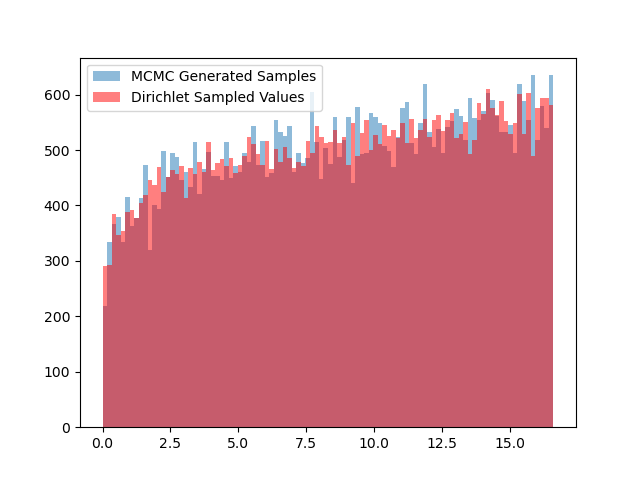
\includegraphics[scale=0.55]{dist.png}
\subsubsection{Ajustando as bordas dinamicamente}
\indent Para que tenhamos bins com peso semelhantes, ou seja, todos próximos a $1/k$ ajustaremos dinamicamente as bordas de cada bin. Para isso, ordenaremos todo o nosso espaço de $f(\theta | x,y)$ em ordem crescente e realizaremos $k$ cortes nesse array, de modo que cada pedaço possuirá $n/k$ membros do vetor de $f(\theta | x,y)$, pegamos então as bordas direitas destes vetores e igualamos a cada ponto $v$.  Deste modo teremos todos os bins balanceados.
\subsubsection{Calculando uma aproximação para W(v)}
\indent Dado que temos todos os bins ajustados e os seus limites calculados precisamos agora criar uma função que corretamente simula o comportamento de W(v). \\ 
\indent Como indicado no enunciado do exercicio, a fração de $f(\theta)$ presentes até um ponto $v_j$ é uma aproximação de $W(v_j)$, chamaremos essa função aproximada de $U(v)$, o que fazemos, para um dado ponto $v$, será somar as frações, ou seja, somar os bins (com suas fração de pontos) até que a borda de um bin seja maior que o $v$ passado para a função
%%%%%%%%%%%%%%%%%%%%%%
%%%%%%%%%%%%%%%%%%%%%%
\section{Implementação e Testes}
%%%%%%%%%%%%%%%%%%%%%%
%%%%%%%%%%%%%%%%%%%%%%
\indent O algoritmo foi implementado na linguagem Python na versão 3.8.8, organizado em 1 arquivo: statisticalModel.py. \\
\indent A álgebra com vetores, assim como a geração de números aleatórios a partir de uma distribuição (no caso a Gamma) foi feita através da biblioteca \textit{NumPy}. O esqueleto do código pode ser encontrado na seção abaixo 
\subsection{Arquivos do Projeto}
\indent Abaixo segue um breve resumo do conteúdo dos códigos fonte e interfaces.
\indent \textbf{statisticalModel.py}: Implementa todo o algoritmo. Separado em duas classes principais. Apresentarei apenas os métodos públicos das classes neste documento.
\begin{lstlisting}
    class Dirichlet(alpha: List[int]):
        def sample() -> List[float]:

    class StatisticalModel(
        observations: List[int],
        prior: List[int],
        cut_off_points: int,
        theta_n_size: int=30000,
    ):
        def calculate_fraction_of_sets() -> Dict[(str, float)]:
        
        def U(v) -> float:
\end{lstlisting}
\subsection{Algoritmo}
\indent Explicando um pouco melhor cada método mais relevante do programa.
\begin{itemize}
    \item \textit{Dirichlet()}
    \begin{itemize}
        \item .sample\_metropolis\_hasting(): retorna uma lista com os valores de theta da distribuição de Dirichlet que modela nosso problema baseado no algoritmo do Metropolis-Hasting, explicado brevemente anteriormente (I.C.2)
    \end{itemize}
\end{itemize}
\begin{itemize}
\item \textit{StatisticalModel()}
    \begin{itemize}
        \item .calculate\_fraction\_of\_sets(): calcula a fração de pontos do espaço de theta criado em cada bin do nosso modelo e retorna um dicionario que mostra o limite inferior e superior de cada bin como chave e a fração nele presente como valor.
        \item .\_adjust\_bounds\_for\_balanced\_bins(): método protegido que é chamado na instanciação da classe. Ele é responsável pelo ajuste dinâmico dos sets de corte.
        \item .U(v): método que aproxima $W(v)$ dado um valor de $v$ e retorna o valor aproximado 
    \end{itemize}
\end{itemize}
\section{Conclusão}
\indent Após diversos testes com diversos valores diferentes de $k$ e $n$, obtivemos um valor agradável de erro por volta de $k = 50000$ e $n = 300000$. \\
\indent Para estes valores o desvio padrão de um mesmo valor rodado diversas vezes com um modelo instanciado com variáveis aleatórias diferentes e independentes entre modelos, atingimos um desvio padrão menor que 0.05, desejado pelo enunciado do exercício. \\
\indent Além disso, para iniciar o modelo estatístico (com o set dinâmico dos limites de cada \textit{bin}) temos uma demora de aproximadamente 40.29 segundos, onde, após a instanciação da classe, demoramos um tempo infimamente menor (2.57 nano segundos, calculado usando o Google Colabs com a utilidade \textit{\%timeit}) para obtermos um valor de $U(v) \approx W(v)$, isso utilizando variáveis de teste que não necessariamente representam o real valor a ser testado.
\end{document}